\documentclass[a4paper,12pt]{article}

\usepackage[utf8]{inputenc}
\usepackage{lmodern}
\usepackage[margin=1cm]{geometry}
\usepackage{amsmath}
\usepackage{graphicx}
\usepackage{xcolor}
\usepackage{caption}
\usepackage{tikz}
\usetikzlibrary{arrows.meta,positioning,shapes.geometric,calc,fit}

\pagestyle{empty}

\begin{document}
\begin{figure}[p]
  \centering
  \makebox[\textwidth][c]{\resizebox{1.08\textwidth}{!}{%
  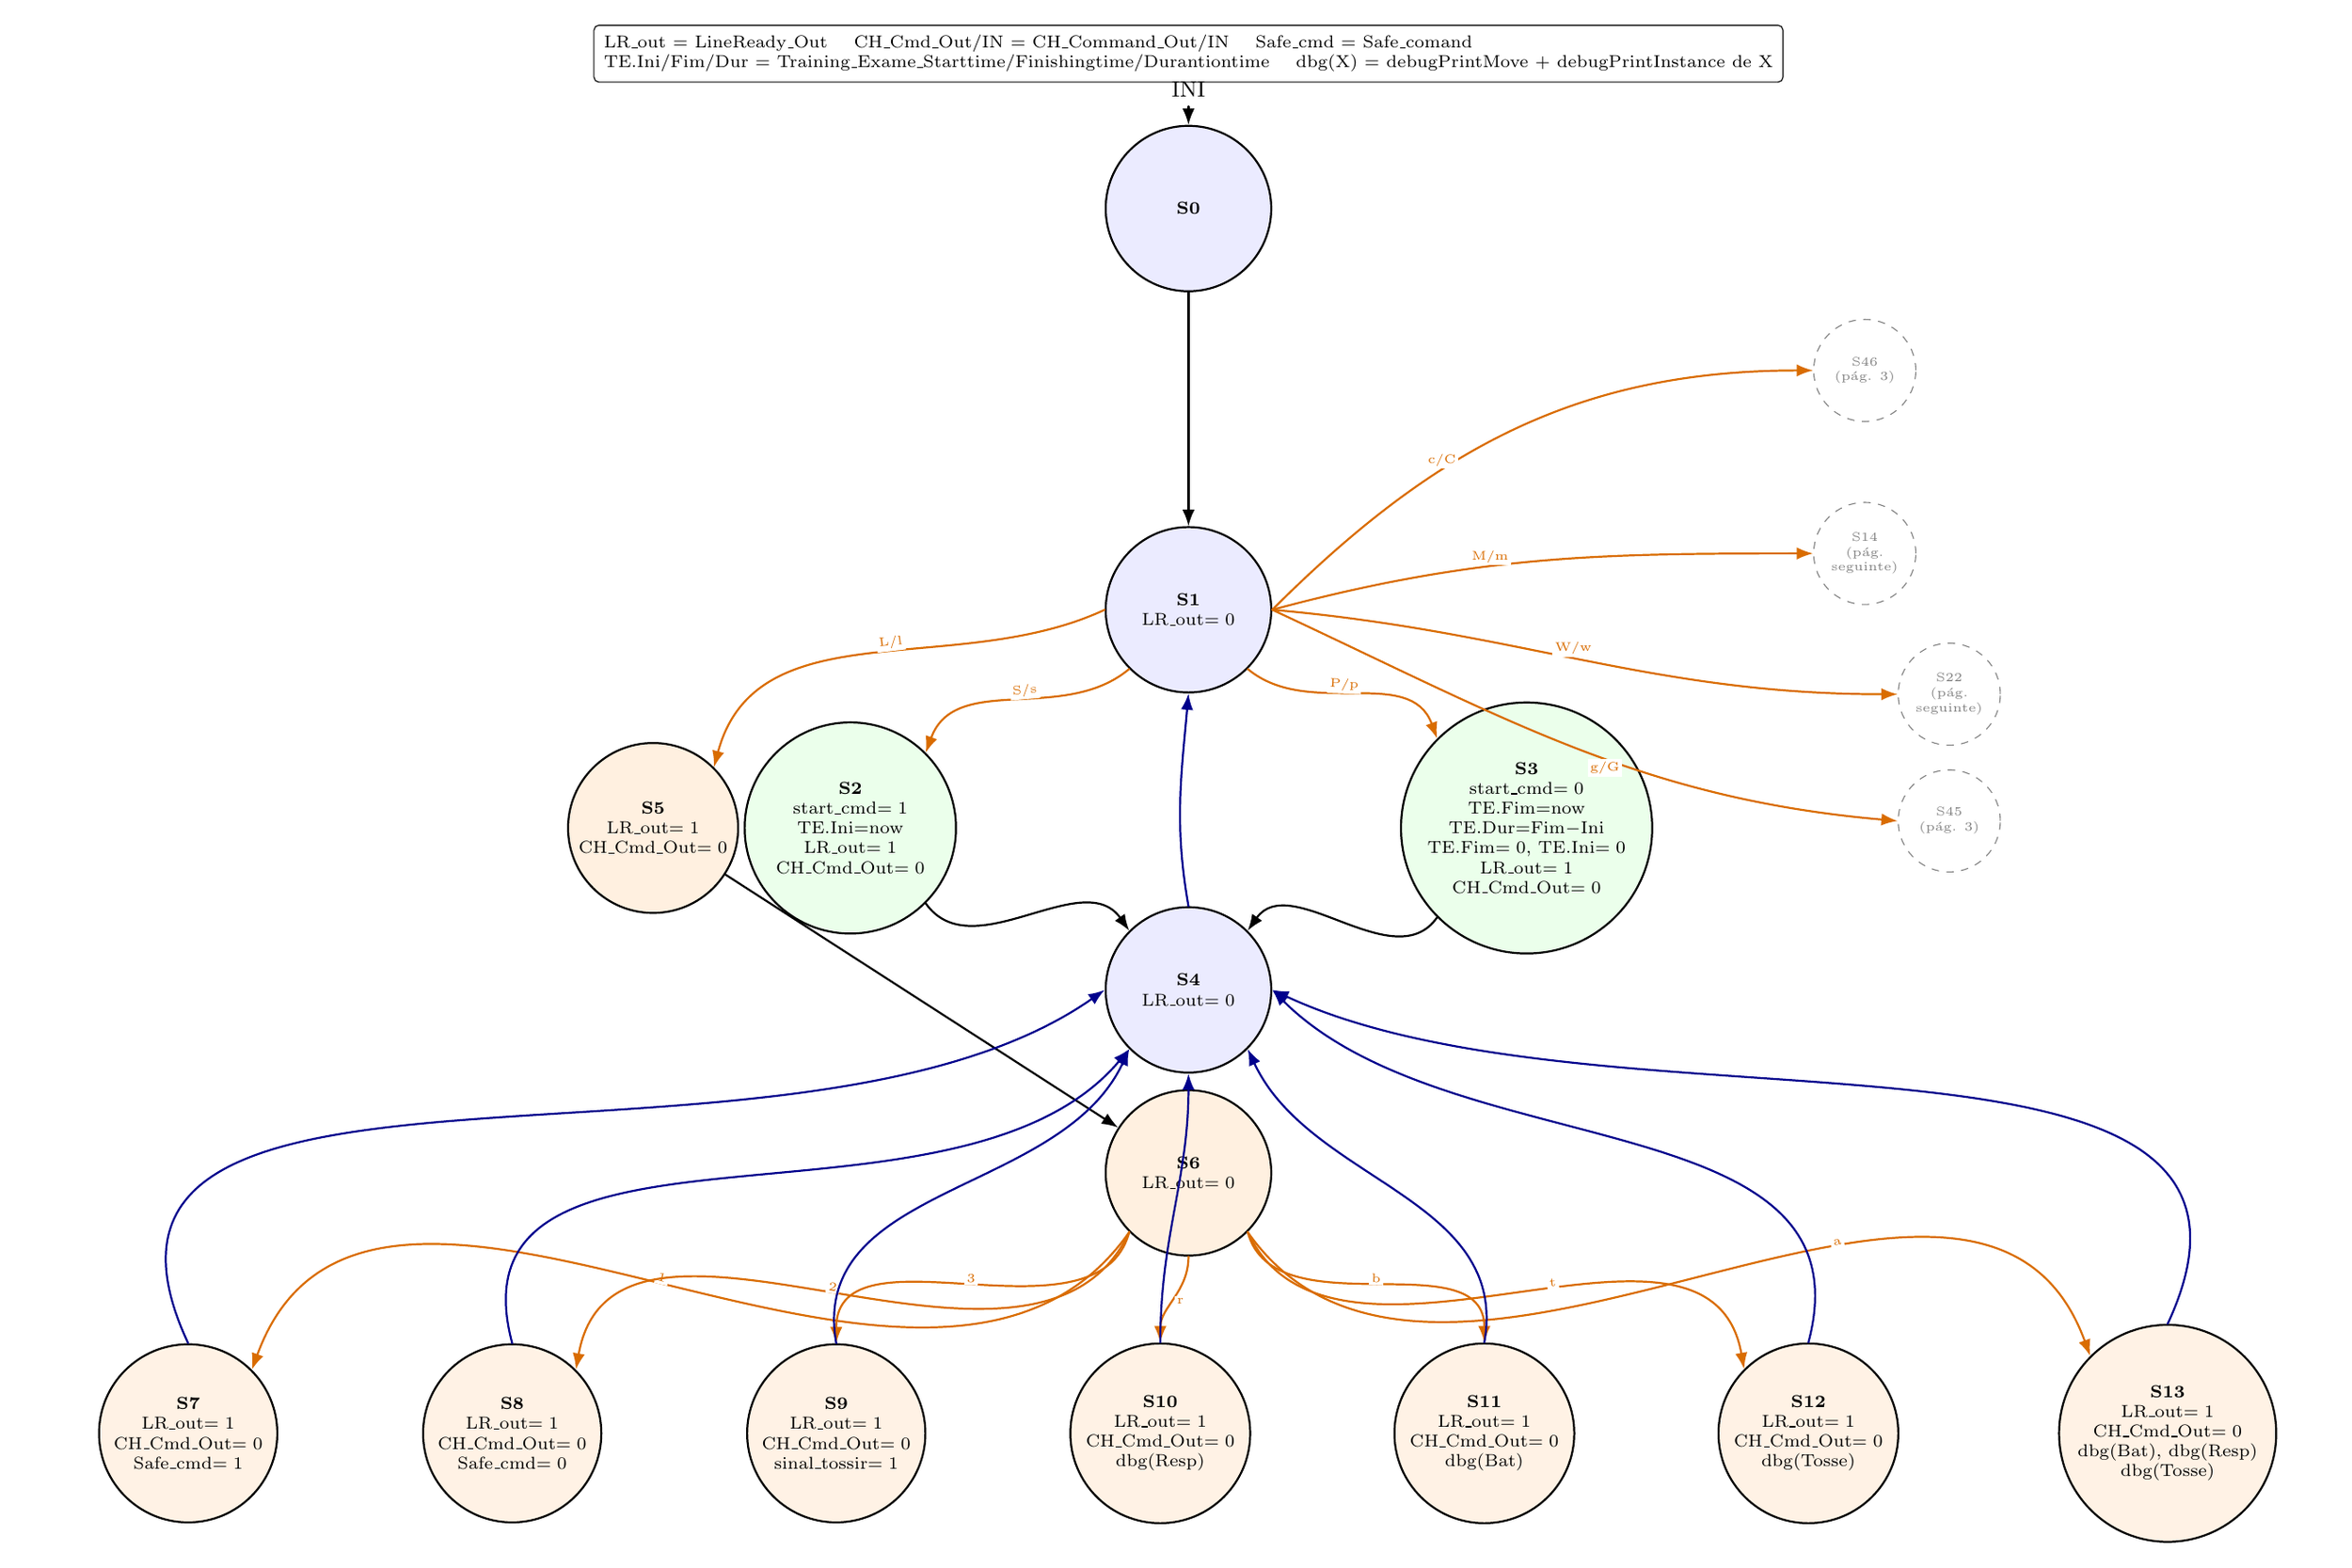
\begin{tikzpicture}[
    x=1cm,
    y=1cm,
    state/.style={draw, circle, align=center, minimum size=2.35cm, inner sep=2pt, font=\scriptsize, thick},
    bigstate/.style={state, minimum size=3.0cm},
    proxy/.style={draw, dashed, circle, align=center, minimum size=1.45cm, font=\tiny, gray},
    arrow/.style={-Latex, thick, line cap=round, line join=round},
    cmd/.style={-Latex, thick, orange!85!black, line cap=round, line join=round},
    ret/.style={-Latex, thick, blue!55!black, line cap=round, line join=round},
    lab/.style={font=\tiny, align=center, fill=white, inner sep=1pt},
    >=Stealth
  ]
    \node[draw, rounded corners=2pt, align=left, font=\scriptsize, inner sep=4pt] at (0,8.7)
      {LR\_out = LineReady\_Out \quad CH\_Cmd\_Out/IN = CH\_Command\_Out/IN \quad Safe\_cmd = Safe\_comand\\
       TE.Ini/Fim/Dur = Training\_Exame\_Starttime/Finishingtime/Durantiontime \quad dbg(X) = debugPrintMove + debugPrintInstance de X};

    \node[state, fill=blue!8] (c0) at (0,6.5) {\textbf{S0}};
    \node[state, fill=blue!8] (c1) at (0,0.8) {\textbf{S1}\\LR\_out$=0$};

    \draw[arrow] (0,7.95) node[above]{\small INI} -- (c0.north);
    \node[bigstate, fill=green!8] (c2) at (-4.8,-2.3) {\textbf{S2}\\start\_cmd$=1$\\TE.Ini$=$now\\LR\_out$=1$\\CH\_Cmd\_Out$=0$};
    \node[bigstate, fill=green!8] (c3) at (4.8,-2.3)  {\textbf{S3}\\start\_cmd$=0$\\TE.Fim$=$now\\TE.Dur$=$Fim$-$Ini\\TE.Fim$=0$, TE.Ini$=0$\\LR\_out$=1$\\CH\_Cmd\_Out$=0$};
    \node[state, fill=blue!8] (c4) at (0,-4.6) {\textbf{S4}\\LR\_out$=0$};
    \node[state, fill=orange!12] (c5) at (-7.6,-2.3) {\textbf{S5}\\LR\_out$=1$\\CH\_Cmd\_Out$=0$};
    \node[state, fill=orange!12] (c6) at (0,-7.2) {\textbf{S6}\\LR\_out$=0$};

    \node[state, fill=orange!10] (c7)  at (-14.2,-10.9) {\textbf{S7}\\LR\_out$=1$\\CH\_Cmd\_Out$=0$\\Safe\_cmd$=1$};
    \node[state, fill=orange!10] (c8)  at (-9.6,-10.9)  {\textbf{S8}\\LR\_out$=1$\\CH\_Cmd\_Out$=0$\\Safe\_cmd$=0$};
    \node[state, fill=orange!10] (c9)  at (-5.0,-10.9)  {\textbf{S9}\\LR\_out$=1$\\CH\_Cmd\_Out$=0$\\sinal\_tossir$=1$};
    \node[state, fill=orange!10] (c10) at (-0.4,-10.9)  {\textbf{S10}\\LR\_out$=1$\\CH\_Cmd\_Out$=0$\\dbg(Resp)};
    \node[state, fill=orange!10] (c11) at (4.2,-10.9)   {\textbf{S11}\\LR\_out$=1$\\CH\_Cmd\_Out$=0$\\dbg(Bat)};
    \node[state, fill=orange!10] (c12) at (8.8,-10.9)   {\textbf{S12}\\LR\_out$=1$\\CH\_Cmd\_Out$=0$\\dbg(Tosse)};
    \node[bigstate, fill=orange!10] (c13) at (13.9,-10.9) {\textbf{S13}\\LR\_out$=1$\\CH\_Cmd\_Out$=0$\\dbg(Bat), dbg(Resp)\\dbg(Tosse)};

    \node[proxy] (p46) at (9.6,4.2)  {S46\\(pág. 3)};
    \node[proxy] (p14) at (9.6,1.6)  {S14\\(pág.\\seguinte)};
    \node[proxy] (p22) at (10.8,-0.4) {S22\\(pág.\\seguinte)};
    \node[proxy] (p45) at (10.8,-2.2) {S45\\(pág. 3)};

    \draw[arrow] (c0) -- (c1);
    \draw[cmd] (c1.south west) to[out=220,in=70] node[lab, pos=0.45, above, sloped]{S/s} (c2.north east);
    \draw[cmd] (c1.south east) to[out=320,in=110] node[lab, pos=0.45, above, sloped]{P/p} (c3.north west);
    \draw[cmd] (c1.west) to[out=205,in=75] node[lab, pos=0.45, above, sloped]{L/l} (c5.north east);
    \draw[cmd] (c1.east) to[out=45,in=180] node[lab, pos=0.35, above]{c/C} (p46.west);
    \draw[cmd] (c1.east) to[out=15,in=180] node[lab, pos=0.40, above]{M/m} (p14.west);
    \draw[cmd] (c1.east) to[out=-5,in=180] node[lab, pos=0.48, above]{W/w} (p22.west);
    \draw[cmd] (c1.east) to[out=-25,in=175] node[lab, pos=0.55, below]{g/G} (p45.west);
    \draw[arrow] (c2.south east) to[out=-55,in=125] (c4.north west);
    \draw[arrow] (c3.south west) to[out=-125,in=55] (c4.north east);
    \draw[ret] (c4.north) to[out=100,in=-95] (c1.south);
    \draw[arrow] (c5) -- (c6);
    \draw[cmd] (c6.south west) to[out=235,in=70] node[lab, pos=0.50, above, sloped]{1} (c7.north east);
    \draw[cmd] (c6.south west) to[out=245,in=80] node[lab, pos=0.50, above, sloped]{2} (c8.north east);
    \draw[cmd] (c6.south west) to[out=255,in=90] node[lab, pos=0.50, above, sloped]{3} (c9.north);
    \draw[cmd] (c6.south) to[out=270,in=90] node[lab, pos=0.52, right]{r} (c10.north);
    \draw[cmd] (c6.south east) to[out=285,in=90] node[lab, pos=0.50, above, sloped]{b} (c11.north);
    \draw[cmd] (c6.south east) to[out=295,in=100] node[lab, pos=0.56, above, sloped]{t} (c12.north west);
    \draw[cmd] (c6.south east) to[out=305,in=110] node[lab, pos=0.64, above, sloped]{a} (c13.north west);
    \draw[ret] (c7.north)  to[out=115,in=215] (c4.west);
    \draw[ret] (c8.north)  to[out=105,in=230] (c4.south west);
    \draw[ret] (c9.north)  to[out=100,in=245] (c4.south west);
    \draw[ret] (c10.north) to[out=90,in=-90] (c4.south);
    \draw[ret] (c11.north) to[out=80,in=-65] (c4.south east);
    \draw[ret] (c12.north) to[out=75,in=-45] (c4.east);
    \draw[ret] (c13.north) to[out=65,in=-25] (c4.east);
  \end{tikzpicture}}}
  \caption{FSM\_Serial\_Command (parte 1 de 3): comandos simples e submenu \texttt{L}.}
  \label{fig:fsm-serial-command-p1}
\end{figure}

\end{document}
